% WACV 2024 Paper Template
% based on the CVPR 2023 template (https://media.icml.cc/Conferences/CVPR2023/cvpr2023-author_kit-v1_1-1.zip) with 2-track changes from the WACV 2023 template (https://github.com/wacv-pcs/WACV-2023-Author-Kit)
% based on the CVPR template provided by Ming-Ming Cheng (https://github.com/MCG-NKU/CVPR_Template)
% modified and extended by Stefan Roth (stefan.roth@NOSPAMtu-darmstadt.de)

\documentclass[10pt,twocolumn,letterpaper]{article}

%%%%%%%%% PAPER TYPE  - PLEASE UPDATE FOR FINAL VERSION
% \usepackage[review,algorithms]{../wacv}      % To produce the REVIEW version for the algorithms track
%\usepackage[review,applications]{wacv}      % To produce the REVIEW version for the applications track
\usepackage{wacv}              % To produce the CAMERA-READY version
%\usepackage[pagenumbers]{wacv} % To force page numbers, e.g. for an arXiv version

% Include other packages here, before hyperref.
\usepackage{graphicx}
\usepackage{amsmath}
\usepackage{amssymb}
\usepackage{booktabs}
\usepackage{xr}

% Include other packages here, before hyperref.
\externaldocument[Supp-]{supplementary_material}

% It is strongly recommended to use hyperref, especially for the review version.
% hyperref with option pagebackref eases the reviewers' job.
% Please disable hyperref *only* if you encounter grave issues, e.g. with the
% file validation for the camera-ready version.
%
% If you comment hyperref and then uncomment it, you should delete
% ReviewTempalte.aux before re-running LaTeX.
% (Or just hit 'q' on the first LaTeX run, let it finish, and you
%  should be clear).
\usepackage[pagebackref,breaklinks,colorlinks]{hyperref}


% Support for easy cross-referencing
\usepackage[capitalize]{cleveref}
\crefname{section}{Sec.}{Secs.}
\Crefname{section}{Section}{Sections}
\Crefname{table}{Table}{Tables}
\crefname{table}{Tab.}{Tabs.}


%%%%%%%%% PAPER ID  - PLEASE UPDATE
\def\wacvPaperID{1891} % *** Enter the WACV Paper ID here
\def\confName{WACV}
\def\confYear{2024}

\begin{document}

%%%%%%%%% TITLE
% title
\title{PETIT-GAN: Physically Enhanced Thermal Images Translation Generative Adversarial Network}	
% author 
% (In the mandatory argument "{}", separate multiple
% authors with "\and" - use "\\" for better author name formatting
% in the title page. In the optional argument "[]" include all
% author names, with no "\and" or text formatting macros.)
% Example: 
%\author[A. Author Albert Einstein]{Anthony Author \and Albert Einstein}
\author[Omri Berman Dr. Iftach Klapp Navot Oz]{Omri Berman \\[.2cm]{\scriptsize Navot Oz \qquad Prof. David Mendlovic \qquad Dr. Iftach Klapp}}
% Address
%  \subtitle{\textsc{Subtitle}}

% \institute{\textsc{Volcani Center} \\
%       Optical Sensing Lab \\
%       [5pt]{\includegraphics[height=3cm,keepaspectratio]{\fulllogovolcani}}
% }
% \institute{\textsc{Tel Aviv University} \\
%       Faculty of Engineering \\
%       [5pt]{\includegraphics[height=3cm,keepaspectratio]{\logotlv}}
% }
\institute{{\includegraphics[height=2cm,keepaspectratio]{\logotlv}}
        \hfill
        {\includegraphics[height=2cm,keepaspectratio]{\fulllogovolcani}}
}

% date
\presentationDate{March 15, 2023}

\begin{frame}[plain]
    \titlepage
\end{frame}
  

%%%%%%%%% ABSTRACT
\begin{abstract}
  The task of image-to-image (I2I) translation involves transforming the style of an image to that of a desired modality while preserving its content.
  In most cases, pairs of content-wise-aligned input-target images are not available, resulting in an unpaired I2I (UI2I) setup.
  Due to the lack of input-target pairs, the UI2I task is ill-posed, resulting in numerous equally satisfactory outputs for a single input.
  However, some data domains have unique properties that tie the input to the output; these can be exploited to reduce this ambiguity.
  We propose PETIT-GAN, a physically enhanced thermal image-translating generative adversarial network to perform UI2I translation between thermal images.
  Our novel approach embeds physically modeled prior information in an UI2I translation to produce outputs with greater fidelity to the target modality.
  We further show that our solution outperforms the current state-of-the-art models at thermal UI2I translation by approximately $50\%$ with respect to the standard metrics, and enjoys a significantly more consistent training procedure.
\end{abstract}


%%%%%%%%% BODY TEXT
\section{Introduction}
\label{sec:introduction}
% \subsection{Motivation}

\begin{frame}{Multi-Spectral Imaging}
  \begin{itemize}
    \item Multiple channels, small bandwidths.
    \item Enables spectral un-mixing (precision agriculture).
    \item Our focus: thermal spectrum ($7-14 \mu m$). 
    \item Cons: Expensive.
  \end{itemize}

  \begin{figure}
    \centering
    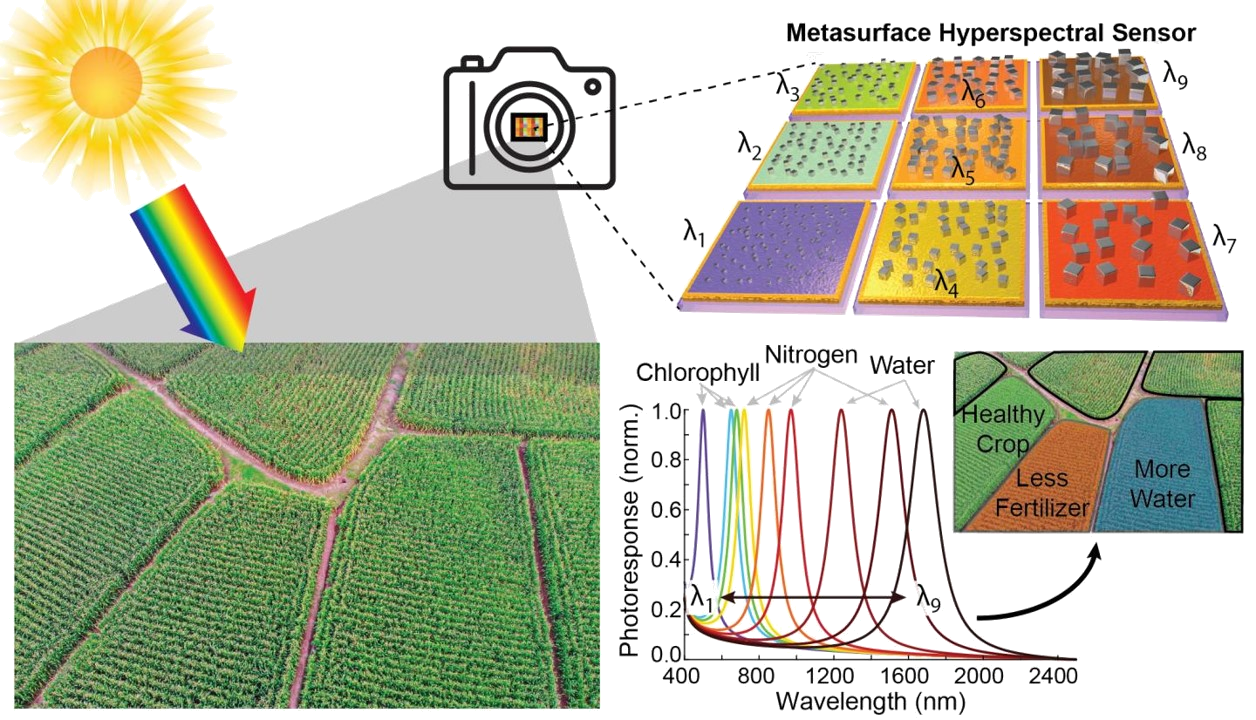
\includegraphics[width=0.6\linewidth]{../figs/introduction/multispectral.png}
  \end{figure}  
\end{frame}

\begin{frame}{Alternative}
    \begin{itemize}
      \item Simpler sensor (cost reduction).
      \item Compensate for compromised quality with CV algorithms.
      \item Deep learning (DL) techniques achieve state-of-the-art (SOTA) results.
      \item Issue: no multispectral thermal data.
    \end{itemize}
  
    \begin{figure}
      \centering
      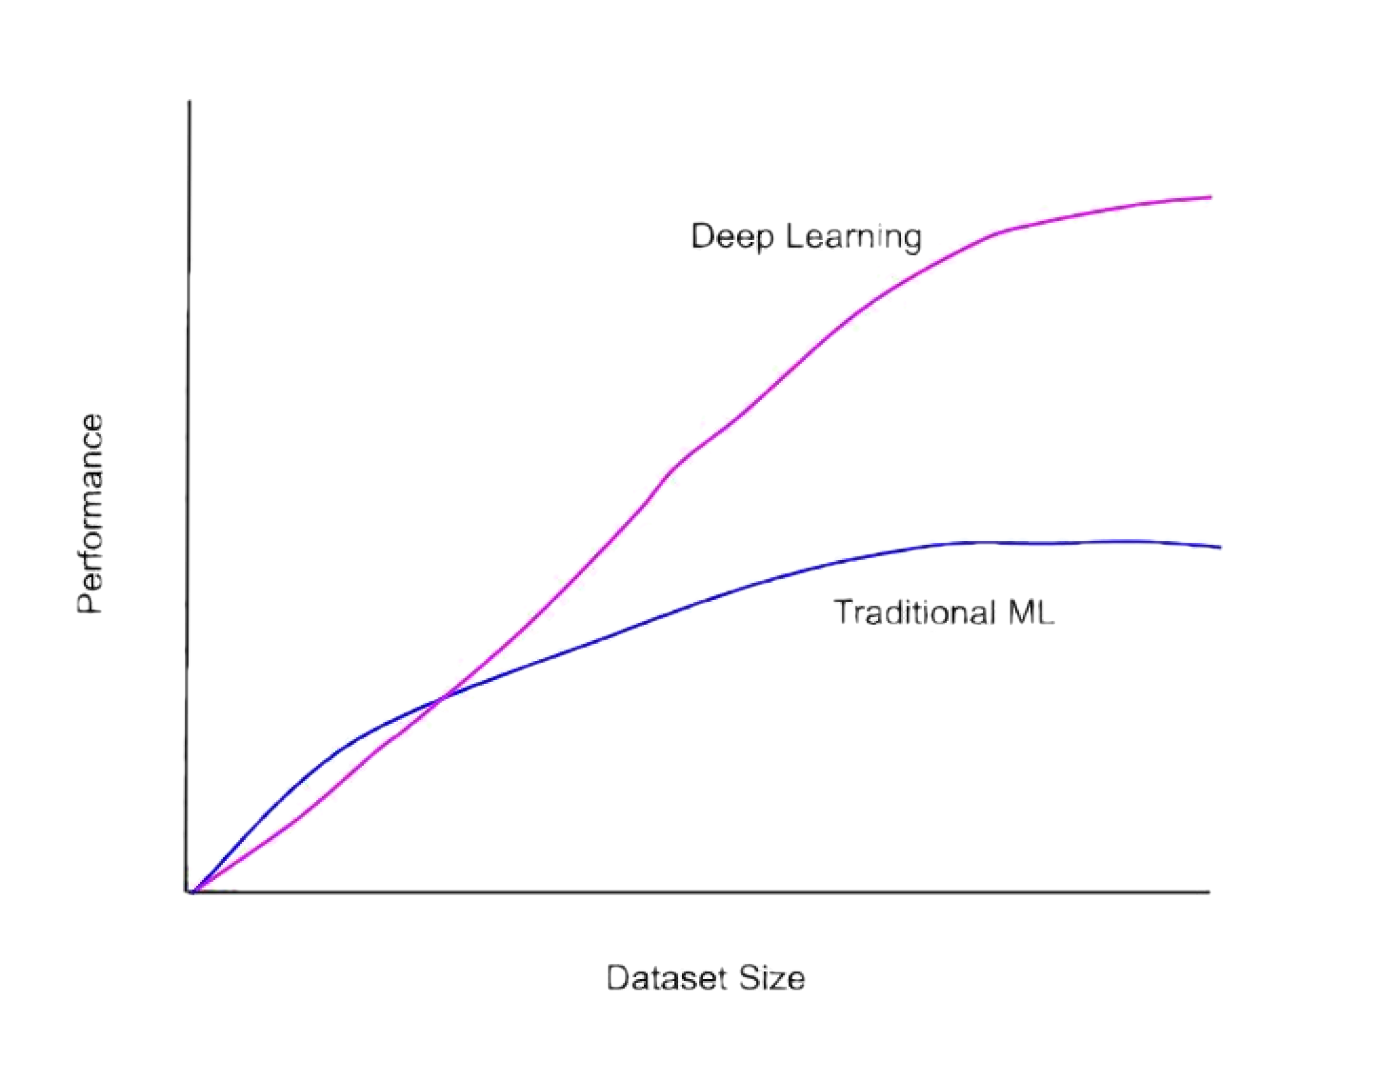
\includegraphics[width=0.5\linewidth]{../figs/introduction/dl_data_requirement.png}
    \end{figure}
  \end{frame}

\begin{frame}{Data Collection}
  \begin{itemize}
        \item Lightweight airplane.
        \item Several flights, each with some IR filter (monochromatic) or without (panchromatic). \hyperlink{apndx:data_collection}{\beamerbutton{More details}}
        \item Issues: registration, small sample size.
    \end{itemize}
    \begin{figure}
        \centering
        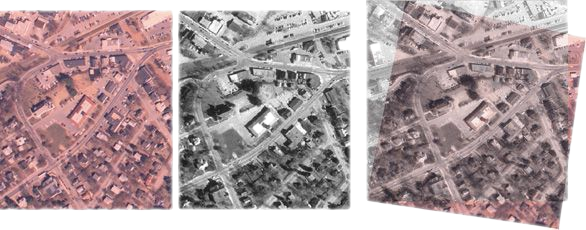
\includegraphics[width=0.8\linewidth]{../figs/introduction/registration.png}
      \end{figure}
  \end{frame}

\begin{frame}{Unpaired Image to Image (UI2I) Generative Models}
  \begin{itemize}
    \item Circumvents the need for \texttt{\textbraceleft} input, target \texttt{\textbraceright} tuples.
    \item Spatially consistent transformation between different modalities.
    \begin{figure}
      \centering
      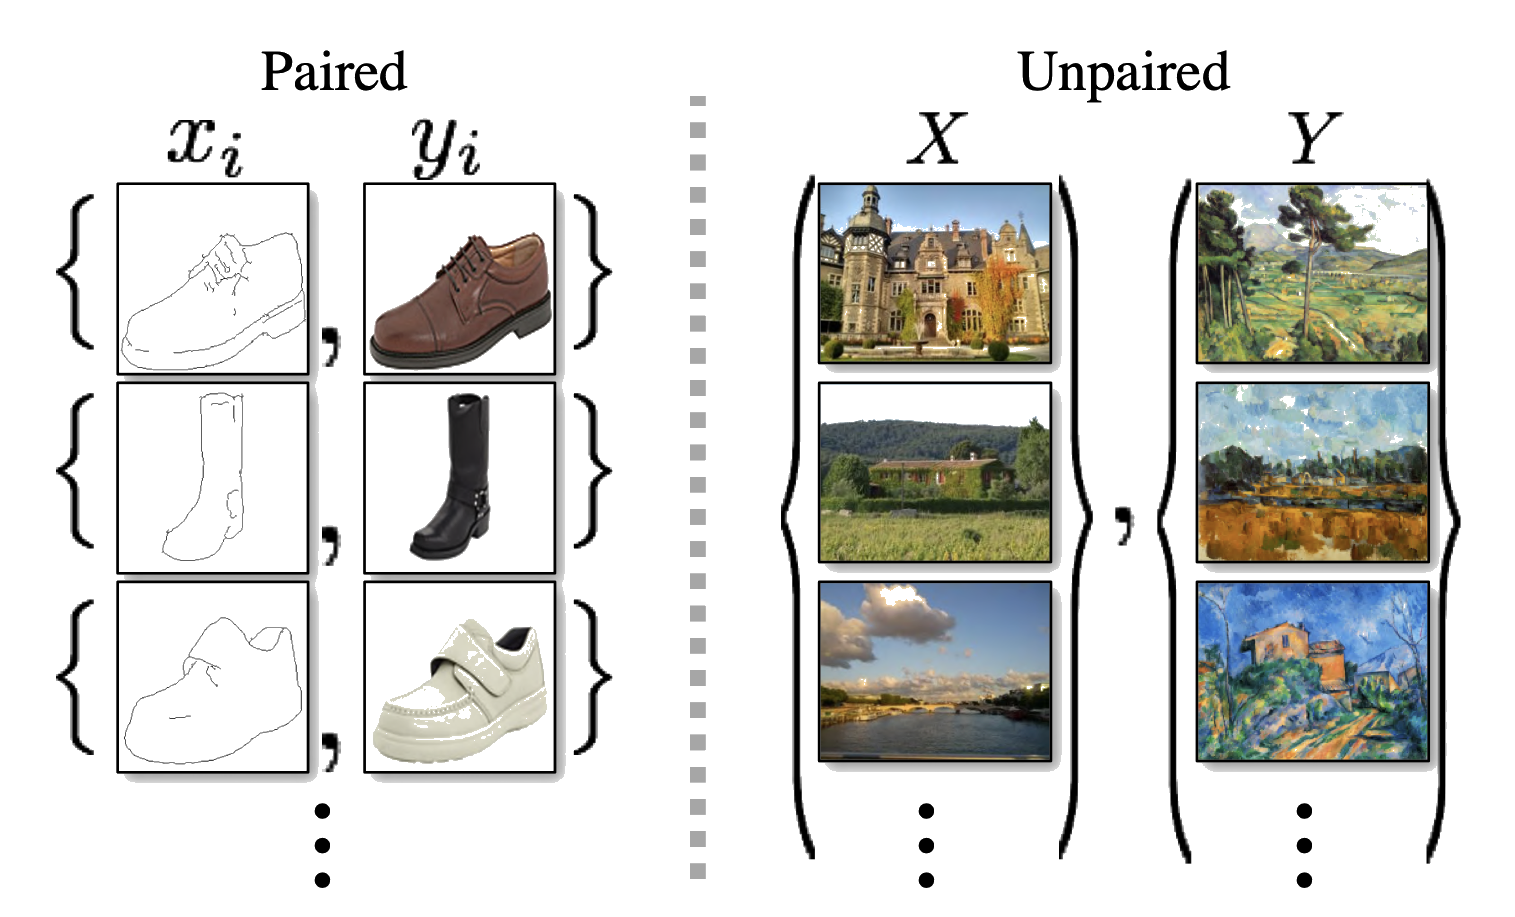
\includegraphics[width=0.7\linewidth]{../figs/related_work/paird_vs_unpaired_I2I.png}
    \end{figure}
  \end{itemize}
\end{frame}

\begin{frame}{Research Motivation}
  \begin{exampleblock}{Goal}
    Learn an UI2I transformation between different thermal spectra.
  \end{exampleblock} 
  \begin{exampleblock}{Hypothesis}
    Unique thermal physics can improve the quality of deep UI2I models.
  \end{exampleblock}  
  \begin{exampleblock}{Showcase}
    Transformation of wide-band (panchromatic) thermal images and to narrow-band (monochromatic) thermal images.
  \end{exampleblock}
\end{frame}

\section{Related work}
\label{sec:related_work}
GAN is a class of deep generative models, first introduced by Goodfellow \etal \cite{goodfellow2014generative}.
Many improvements and extensions have been made in the field of GANs in the last few years, and many of these form the underlying principles and architecture of numerous SOTA models in several generative tasks.
GANs are typically made up of two components: 
(1) a generator, which samples random vectors from some predefined probability density function as inputs and transforms them into meaningful outputs of some target modality; 
(2) a discriminator, which has access to both real images from the target modality and the generator's outputs, and needs to tell them apart.
The generator and discriminator are trained in an adversarial fashion where one's improvement comes at the expense of the other's. 
If successful, the training procedure converges when the generator and discriminator reach a Nash equilibrium \cite{goodfellow2014generative}.

Among the various tasks performed by GANs is I2I translation, where the output is conditioned on an input image.
I2I translation has a plethora of applications, such as image segmentation \cite{yang2018mri, li2020simplified}, pose estimation \cite{li2020manigan, fish2017adversarial}, colorization \cite{isola2017image, suarez2017infrared, zhang2017real}, super resolution \cite{yuan2018unsupervised, zhang2019multiple} and many more.
The I2I translation task can be roughly classified into supervised I2I (paired I2I), where each image in the input domain has a content-aligned equivalent in the output domain, and unsupervised I2I (UI2I), where there are no content-equivalent pairs in the input and output domains.
Most practical I2I tasks are performed in an unsupervised fashion, as fully registered pairs of images in two different modalities are extremely difficult to obtain.

The great challenge in UI2I translation is that no ground truth is available as a reference for the transformed output.
Thus, in contrast to paired I2I, pixel-level loss cannot be used to steer the training toward a better content-preserving solution.
Therefore, content preservation of the transformation must be enforced by an alternative mechanism.
The most popular strategy to ensure content preservation is to use cycle consistency \cite{Lee_2018_ECCV}.
This approach relies on two translators: one from domain A to domain B ($G_{A \rightarrow B}$), and one in the opposite direction ($G_{B \rightarrow A}$). 
In addition to the standard adversarial loss, a cycle-consistency loss is used to penalize for discrepancies between input $x_A$ and its reconstruction by the roundtrip transformation from A to B and then back to A:
\begin{equation}
    \mathcal{L}_{cyc} = \mathcal{L}\left( x_A, G_{B \rightarrow A} \left( G_{A \rightarrow B}(x_A) \right) \right)
\end{equation}
CycleGAN \cite{CycleGAN2017}, along with DiscoGAN \cite{kim2017learning} and DualGAN \cite{yi2017dualgan}, additionally impose cycle consistency over images originating in domain B, resulting in two simultaneous cyclic losses.

While successfully eliminating the need for ground truth, cycle consistency inherently encourages the transformation to encode information about the input that serves solely for the purpose of cyclic reconstruction.
This encoded information comes at the expense of fidelity to the target modality, which is clearly undesirable.
In an attempt to eliminate the need for cycle consistency, several approaches have implemented a one-sided translation that manages to preserve content in a different fashion.
Typically, this is done by embedding both input and target in some shared style-agnostic space. 
The geometric distance between the embeddings is treated as a measure of content discrepancy, and then minimized to improve content preservation.
Fu \etal \cite{fu2019geometry} encouraged preservation of the geometric relationship between an input and its geometrically transformed versions and their outputs. 
Both F-LSeSim \cite{zheng2021spatially} and contrastive unpaired translation (CUT) \cite{park2020cut} used contrastive representation learning by maximizing the similarity between pairs of corresponding patches in the input and output, and minimizing it for non-matching patches.

\section{Proposed method}
\label{sec:methods}

\begin{frame}{Overview}
  Our UI2I transformation consists of:
  \begin{enumerate}
    \item A deep UI2I estimator (GAN).
    \item A physical estimator calibrated to perform thermal UI2I.
    \item Fusion of deep and physical estimators (PETIT-GAN).
  \end{enumerate}
\end{frame}

\subsection{Deep Estimator}
\begin{frame}{Models}
  \begin{itemize}
    \item Generative Adversarial Networks(GANs):
    \begin{enumerate}
      \item CycleGAN \cite{CycleGAN2017} (cycle consistency).
      \item Contrastive Unpaired Translation (CUT) \cite{park2020cut} (contrastive learning).
    \end{enumerate}
    \item Both models share the same generator implementation.
  \end{itemize}
  \begin{figure}
    \centering
    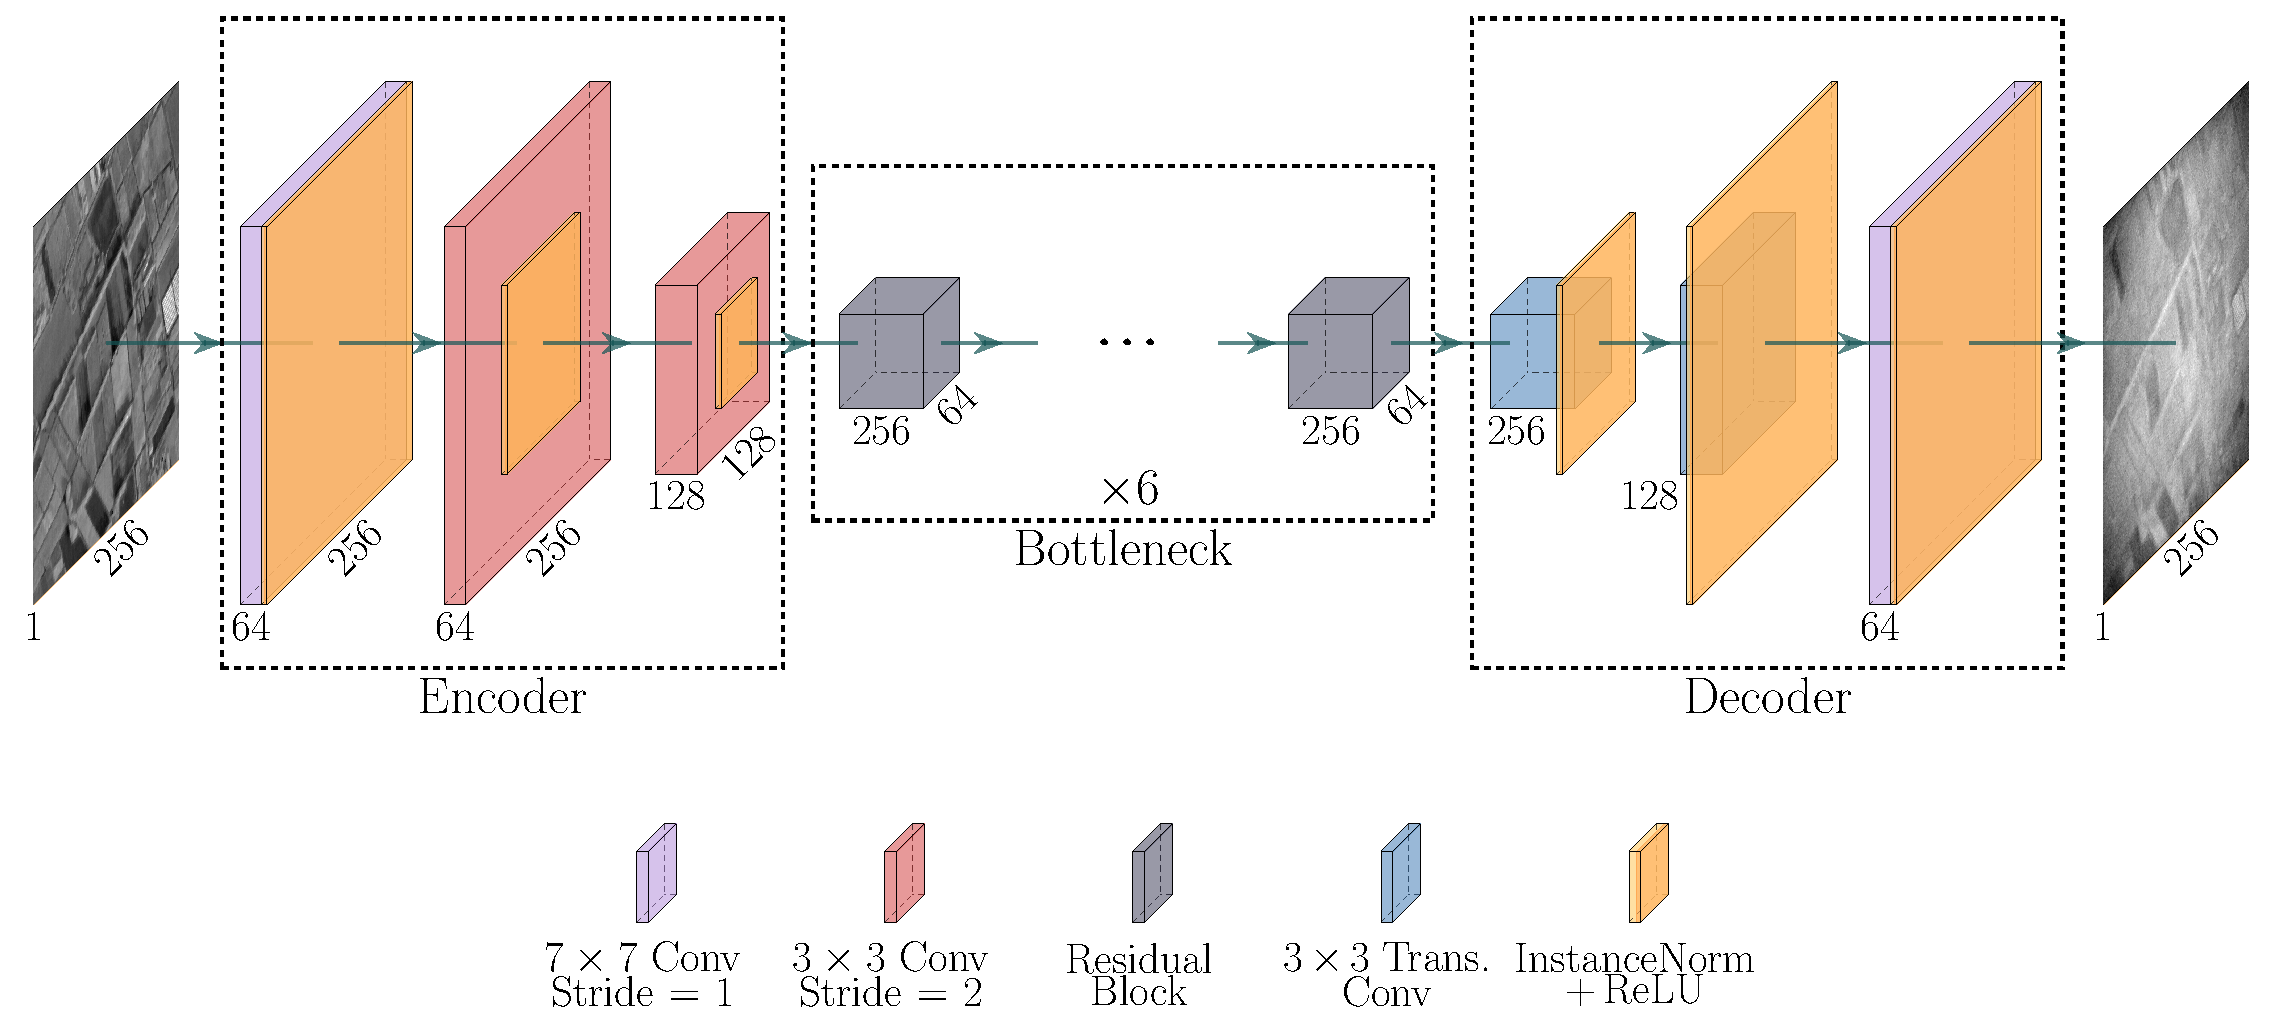
\includegraphics[width=0.7\linewidth]{../figs/network/src/cut.pdf}
  \end{figure}
\end{frame}

\subsection{Physical Estimator}

\begin{frame}{Thermal Imaging}
  \begin{itemize}
    \begin{exampleblock}{Stephan-Boltzmann}
      \begin{equation*} \label{eq:stephan-boltzmann-ideal}
        I(T_\mathit{obj}) = \int_0^\infty \frac{2\pi hc^2}{\lambda^5}\frac{1}{e^{\frac{hc}{\lambda kT_\mathit{obj}}} - 1} d\lambda = \frac{\sigma}{\pi} T_\mathit{obj}^4 \; \; \left[W sr^{-1} m^{-2}\right]
      \end{equation*}
    \end{exampleblock}  
    \item Nugent et al. \cite{10.1117/1.OE.52.6.061304}: dependency on the camera's intrinsic temperature ($T_\mathit{int}$) through 3rd order polynomials:
    \begin{equation*} \label{eq:IntensityVsTemperatures}
      \begin{split}            
        I(T_\mathit{obj}, T_\mathit{int}) &= p^{(0)}_c(T_\mathit{int}) T^4_\mathit{obj} + p^{(1)}_c(T_\mathit{int})\\
        p^{(i)}_c(T_\mathit{int}) &= \sum_{k=0}^3  c_{i,k} T_\mathit{int}^k
    \end{split}
    \end{equation*}
  \end{itemize}
\end{frame}

\begin{frame}{Physical UI2I (Our Contribution)}
  \begin{columns}   
    \begin{column}{0.5\textwidth}
      \begin{itemize} 
        \item Calibrate 2 thermal transformations:
        \begin{enumerate}
          \item $I_\mathit{pan}, T_\mathit{pan} \Rightarrow \hat{T}_\mathit{obj}$ \vspace{0.15cm}
          % \begin{equation*}
          %   \hat{T}_\mathit{obj} = \sqrt[\leftroot{5} 4]{\frac{\pmb{I_\mathit{pan}} - p^{(0)}_{c_\mathit{pan}}(\pmb{T_\mathit{pan}})}{p^{(1)}_{c_\mathit{pan}}(\pmb{T_\mathit{pan}})}}
          % \end{equation*}
          \item $\hat{T}_\mathit{obj}, T_\mathit{mono} \Rightarrow \hat{I}_\mathit{mono}$\vspace{0.25cm}
          % \begin{equation*}
          %   \hat{I}_\mathit{mono} = p^{(1)}_{c_\mathit{mono}}(\pmb{T_\mathit{mono}}) \pmb{\hat{T}_\mathit{obj}}^4 + p^{(0)}_{c_\mathit{mono}}(\pmb{T_\mathit{mono}})
          % \end{equation*}
        \end{enumerate}
        \item Cascade the transformations to get a complete panchromatic to monochromatic UI2I model: 
        \begin{equation*}
          I_\mathit{pan} \Rightarrow \hat{I}_\mathit{mono} 
        \end{equation*}
      \end{itemize}
    \end{column} 
    \begin{column}{0.5\textwidth}
      \begin{figure}            
        \centering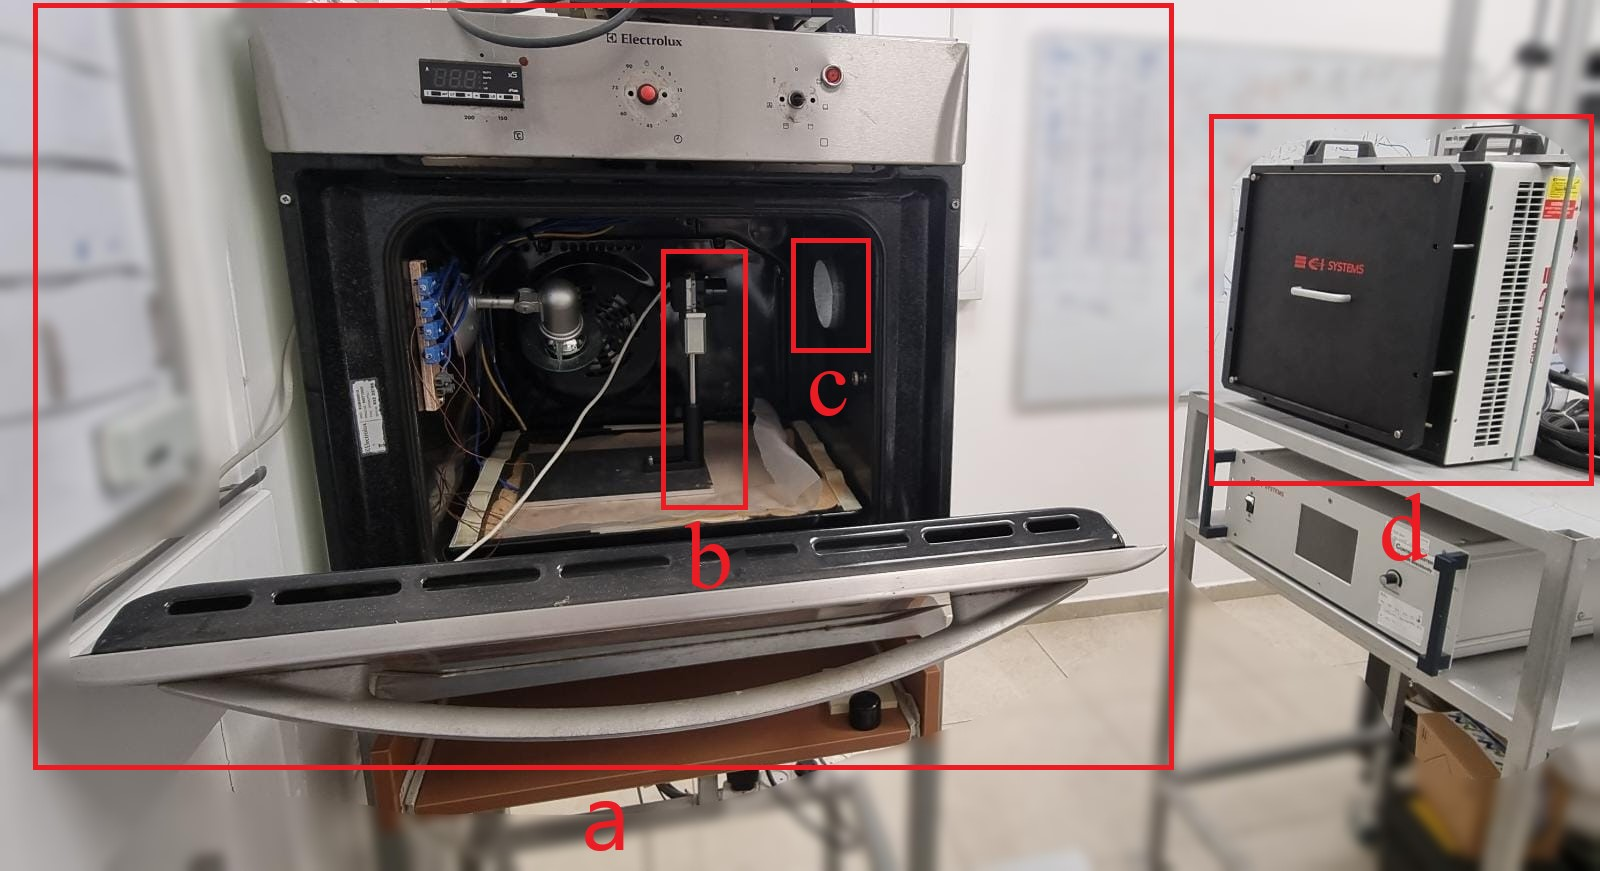
\includegraphics[width=0.75\textwidth]{../figs/methods/calib_setup.jpg}
        \caption*{Calibration Setup}
      \end{figure}      
      
    \end{column} 
  \end{columns}
\end{frame}

\subsection{PETIT}
\begin{frame}{Fusion of Estimators}
  \begin{figure}
    \centering
    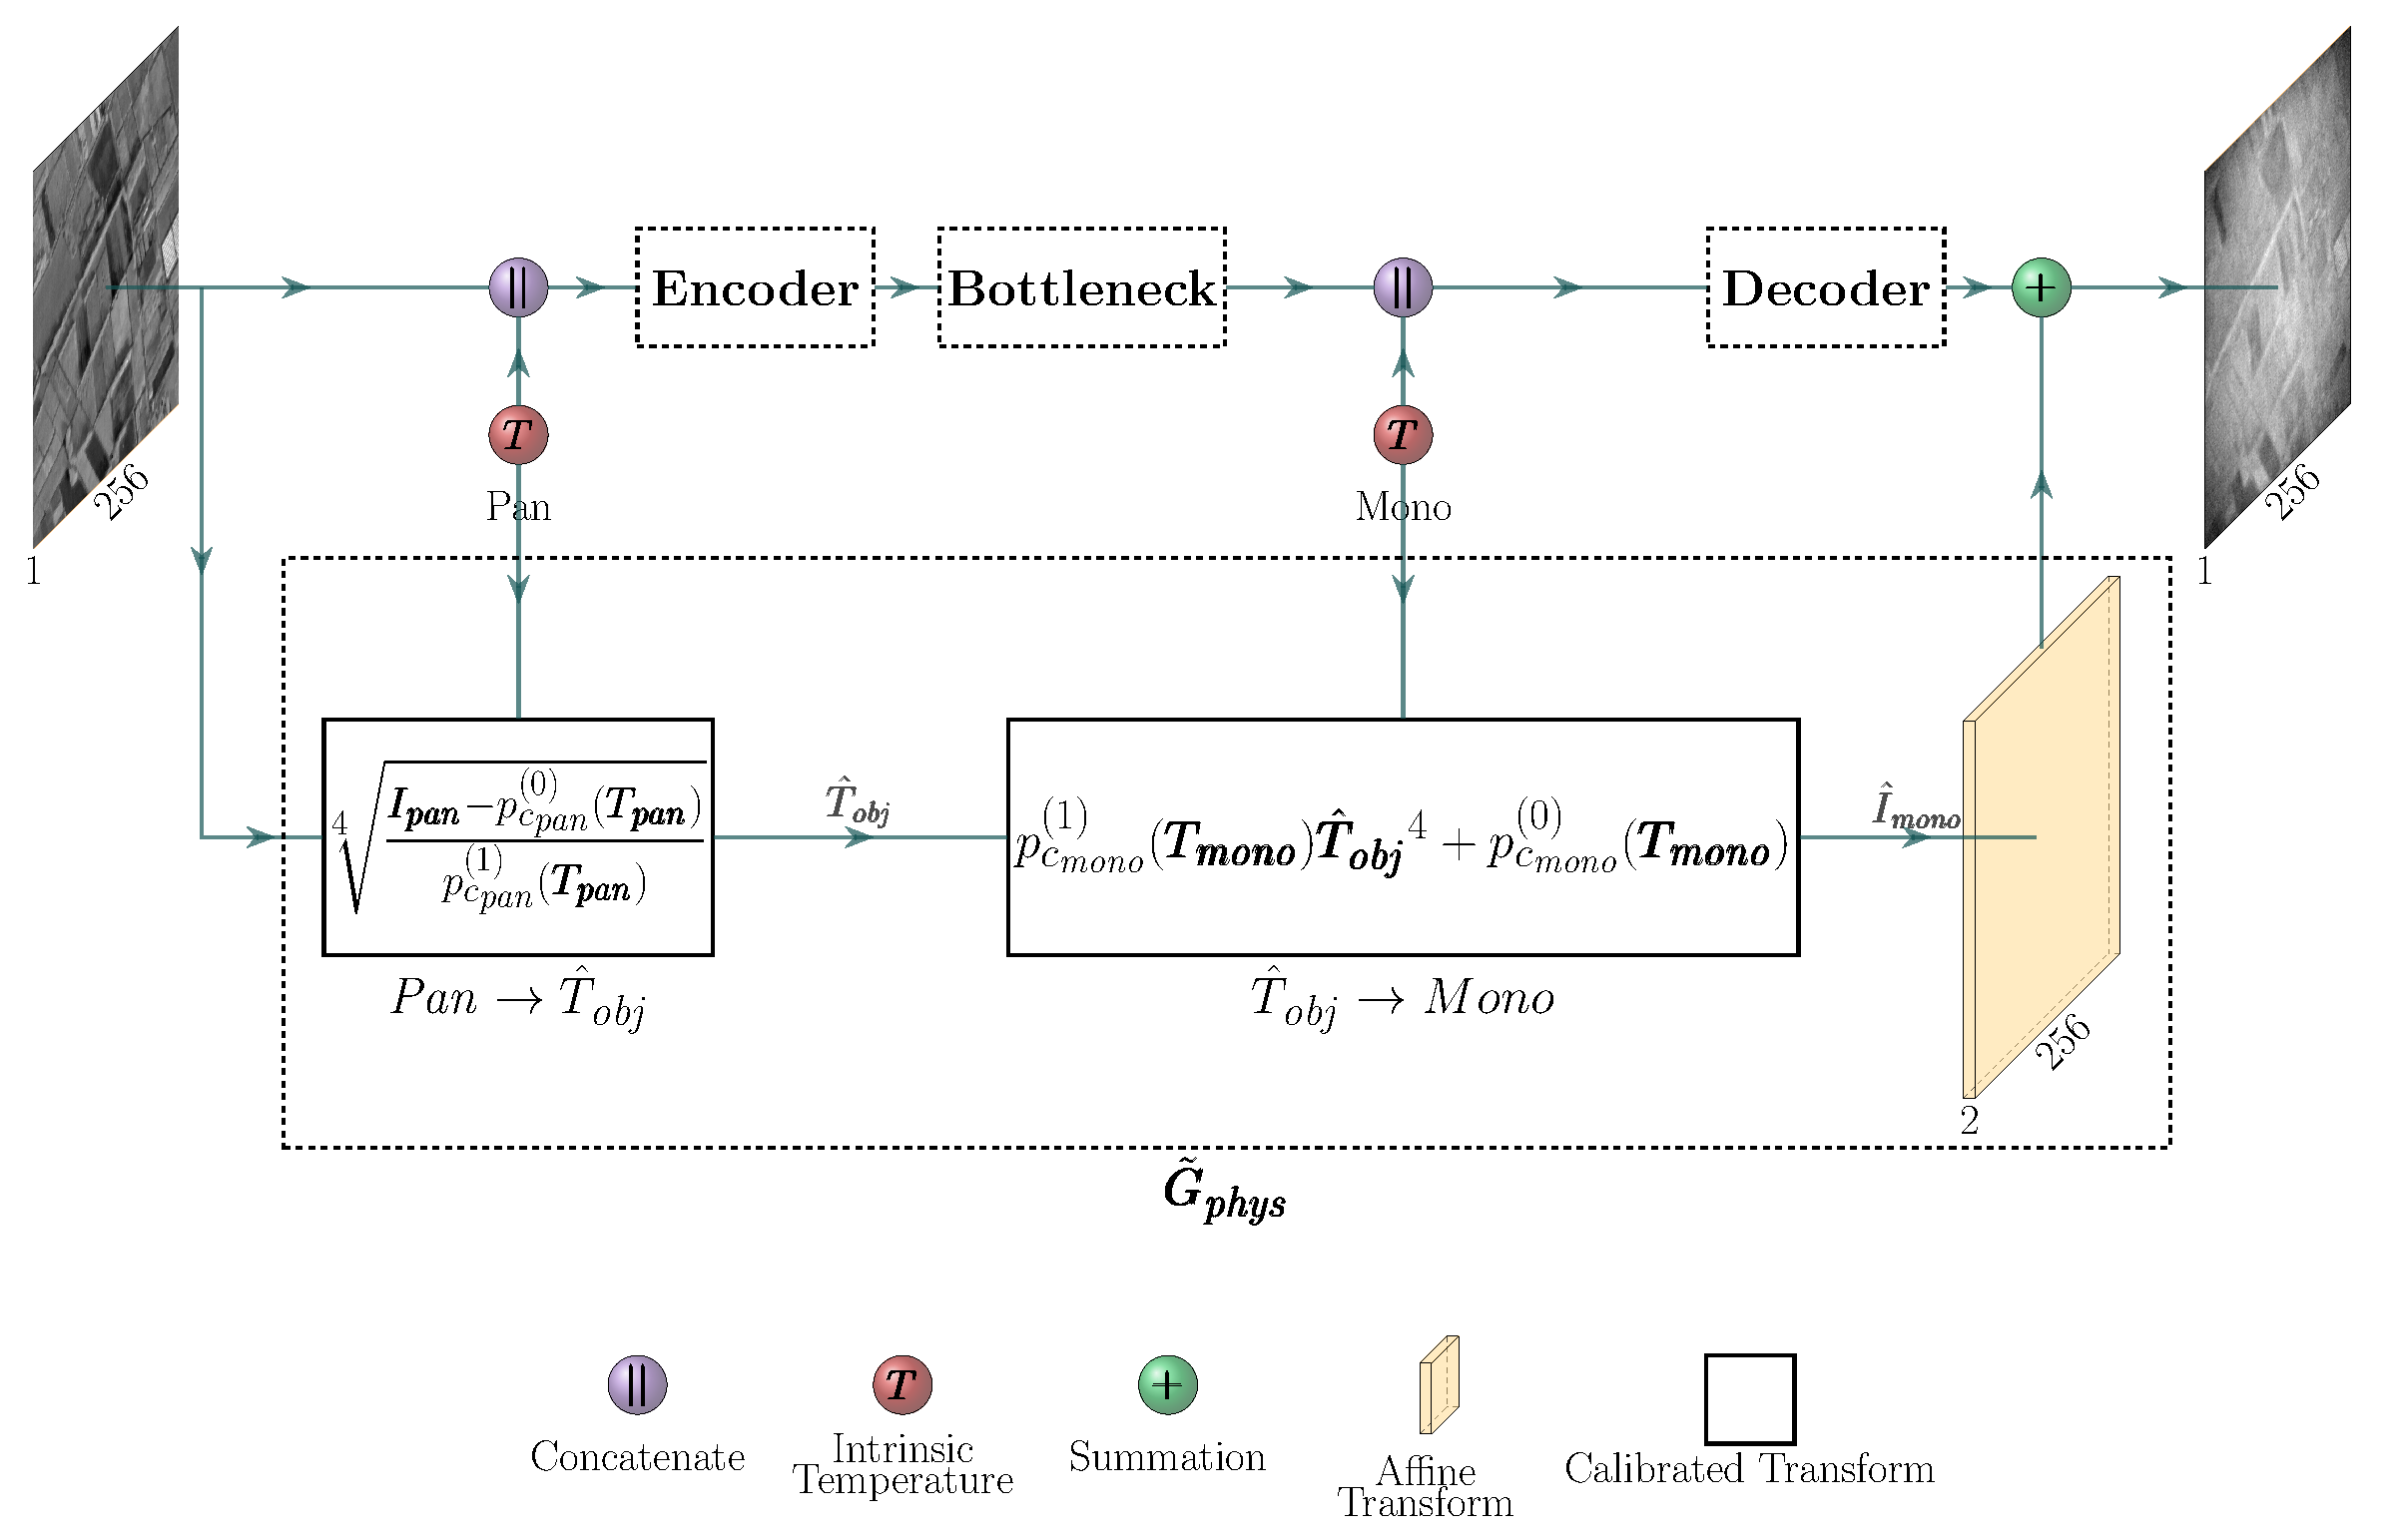
\includegraphics[width=0.65\linewidth]{../figs/network/src/petit.pdf}
  \end{figure}
\end{frame}


\section{Experiments}
\label{sec:experiments}
\begin{frame}{Quantitative}
    \begin{itemize}
      \item Our method was compared to the generative models baselines trained to perform the task end-to-end.
      \item Fréchet Inception Distance (FID) \cite{DBLP:journals/corr/HeuselRUNKH17} metric was used for evaluation.
      \item Each configuration was trained $\times 10$ times and the mean and std were used for comparison.
    \end{itemize}
    \begin{table}
        \centering
        \begin{tabular}{| c  c  || c  c |}
            % \toprule
            \multicolumn{2}{c}{Configuration} & \multicolumn{2}{c}{FID} \\
            % \hline\hline
            \hline
            % \midrule
            Backbone & Caption & Mean & Std\\
            \hline
            \multirow{2}{4em}{CycleGan}  & end-to-end    & 51.05             & 9.82\\      
                                         & PETIT (ours)       & \textbf{33.8}     & \textbf{1.23}\\
            \hline
            \multirow{2}{4em}{CUT}       & end-to-end    & 38.43             & 1.52\\
                                         & PETIT (ours)       & \textbf{27.35}    & \textbf{1.01}\\
            \hline
            % \bottomrule
        \end{tabular}
    \end{table}    
\end{frame}

\begin{frame}{Qualitative}
    \begin{figure}
        % 1st Row
        \centering
        \begin{subfigure}[b]{0.24\textwidth}
            \centering
            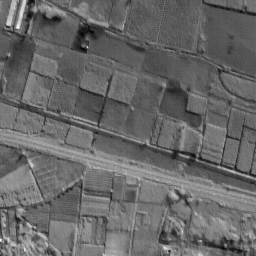
\includegraphics[width=\textwidth]{../figs/outputs/pan/71.png}
        \end{subfigure}
        \hfill
        \begin{subfigure}[b]{0.24\textwidth}
            \centering
            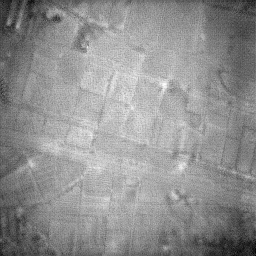
\includegraphics[width=\textwidth]{../figs/outputs/cut/71.png}
        \end{subfigure}
        \hfill
        \begin{subfigure}[b]{0.24\textwidth}
            \centering
            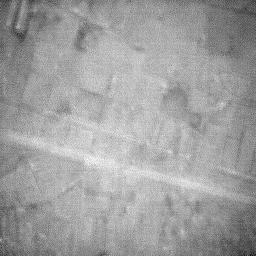
\includegraphics[width=\textwidth]{../figs/outputs/petit/71.png}
        \end{subfigure}
        \hfill
        \begin{subfigure}[b]{0.24\textwidth}
            \centering
            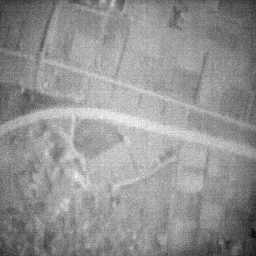
\includegraphics[width=\textwidth]{../figs/outputs/mono/605.png}
        \end{subfigure}      
                
        % 2nd Row
        \begin{subfigure}[b]{0.24\textwidth}
            \centering
            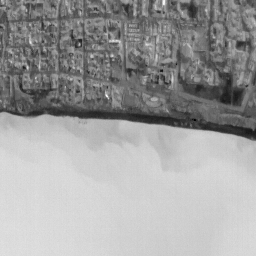
\includegraphics[width=\textwidth]{../figs/outputs/pan/28.png}
            \subcaption{Pan (input)}
            \label{fig:pan}
        \end{subfigure}
        \hfill
        \begin{subfigure}[b]{0.24\textwidth}
            \centering
            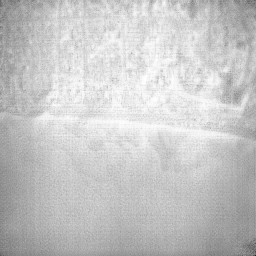
\includegraphics[width=\textwidth]{../figs/outputs/cut/28.png}
            \subcaption{CUT (baseline)}
            \label{fig:cut}
        \end{subfigure}
        \hfill
        \begin{subfigure}[b]{0.24\textwidth}
            \centering
            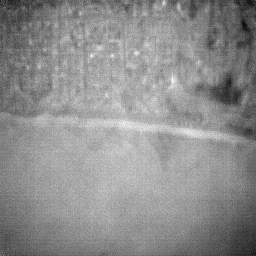
\includegraphics[width=\textwidth]{../figs/outputs/petit/28.png}
            \subcaption{PETIT (ours)}
            \label{fig:petit}
        \end{subfigure}
        \hfill
        \begin{subfigure}[b]{0.24\textwidth}
            \centering
            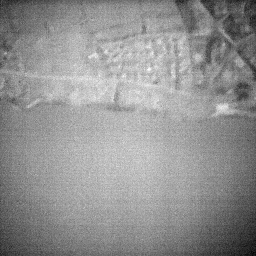
\includegraphics[width=\textwidth]{../figs/outputs/mono/994.png}
            \subcaption{Mono (ref)}
            \label{fig:mono}
        \end{subfigure}
    
        \label{fig:qual_comp}
    
    \end{figure}
\end{frame}

\section{Summary and conclusions}
\label{sec:conclusions}
\begin{frame}{Conclusions}
    \begin{itemize}
      \item Physical modeling is beneficial for thermal UI2I translation. 
      \item PETIT beats deep SOTA UI2I models both quantitatively (by $\approx 50\%$!) and qualitatively.
      \item Fidelity of generated monochromatic images is good enough for synthesizing an artificial multispectral dataset.
    \end{itemize}
\end{frame}


\section*{Acknowledgements}
\label{sec:acknowledgements}
This work has been supported by the Israeli ministry of science and technology, research number 3-17381.


\clearpage
{\small
\bibliographystyle{../ieee_fullname}
\bibliography{../bib}
}

\end{document}